%%=============================================================================
%% Methodologie
%%=============================================================================

\chapter{\IfLanguageName{dutch}{Methodologie}{Methodology}}%
\label{ch:methodologie}

% Door de vergaarde kennis uit de literatuurstudie in hoofdstuk \ref{ch:stand-van-zaken} over de mogelijke noden van scholieren met dyslexie, de complexiteit van wetenschappelijke artikelen, de technieken voor MTS en ATS, en de bijhorende valkuilen bij taalverwerking met AI, kunnen onderzoeksmethoden worden toegepast om een antwoord te vinden op de onderzoeksvraag. 

Om een antwoord te vormen op de onderzoeksvraag, moet de vergaarde kennis uit de literatuurstudie in drie onderzoeksmethoden. Zo doelt dit onderzoek om een prototype te ontwikkelen voor gepersonaliseerde ATS die wetenschappelijke artikelen vereenvoudigd voor scholieren met dyslexie in de derde graad van het middelbaar onderwijs. Eerst staat het onderzoek stil bij de vereiste functionaliteiten. Vervolgens achterhaalt het onderzoek het geschikte taalmodel voor gepersonaliseerde ATS. Tenslotte volgt de ontwikkeling van een prototype voor ATS-vereenvoudiging van .

\section{Requirementsanalyse}
\label{sec:requirementsanalyse}

Om het ontwikkelingsproces van het prototype gericht te sturen, moet het onderzoek MTS- en ATS-technologieën in bestaande tools nagaan. Zo gebeurt het verkennen en experimenteren op ATS-technieken bij beschikbare tools door een kwalitatief onderzoek in de vorm van een requirementsanalyse. Het resultaat van deze onderzoeksfase is een Moscow-schema dat de benodigde functionaliteiten voor een toepassing met ATS definieert, met als doel een vergelijkbare toepassing aan te bieden voor gepersonaliseerde ATS van wetenschappelijke artikelen met de kwaliteiten van gepersonaliseerde MTS. Daarnaast achterhaalt de onderzoeksfase de ontbrekende MTS-functionaliteiten die tabel \ref{table:benefits-mts} in de literatuurstudie uitwees. De geteste toepassingen, opgesomd in tabel \ref{table:shortlist-tools}, beschikken over (gepersonaliseerde) ATS-technieken. Deze lijst omvat erkende toepassingen van de overheid en toepassingen die leerkrachten of scholieren kunnen gebruiken om teksten te vereenvoudigen. Met deze onderzoeksmethode kan het onderzoek een antwoord geven op de volgende twee deelvragen van het onderzoek.

\begin{itemize}
	\item Welke functies ontbreken AI-toepassingen om geautomatiseerde tekstvereenvoudiging mogelijk te maken voor scholieren met dyslexie in de derde graad middelbaar onderwijs?
	\item Welke manuele methoden voor tekstvereenvoudiging komen niet in deze tools voor?
\end{itemize}

Zo vereist de requirementsanalyse een bedachtzame aanpak, weergegeven op de flowchart op figuur \ref{img:flowchart-requirementsanalyse}.

\begin{figure}[H]
	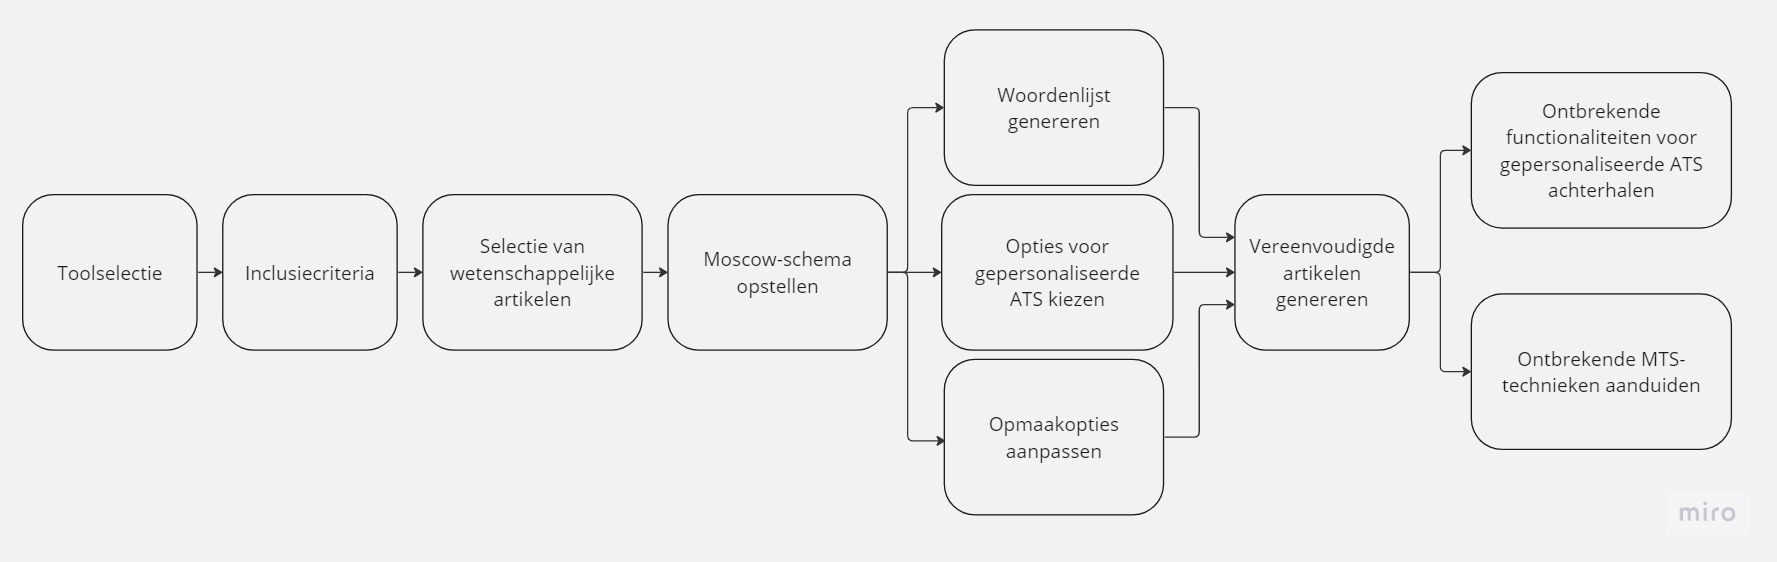
\includegraphics[width=\linewidth]{img/flowchart-requirementsanalyse.jpg}
	\caption{Het benodigde stappenplan bij de requirementanalyse.}
	\label{img:flowchart-requirementsanalyse}
\end{figure}

% TOOLSELECTIE 
Allereerst start het onderzoek met een toolselectie. Zoals aangewezen in sectie \ref{sec:beschikbare-tools-en-taalmodellen}, leent de overheid vijf softwarepakketten uit aan middelbare scholen. Echter zal de requirementsanalyse drie van deze vijf in de analyse opnemen, want hun functionaliteiten zijn toepasselijk voor deze casus. Naast deze softwarepakketten kunnen online beschikbare tools ook scholieren met dyslexie ondersteunen bij het begrijpend lezen van wetenschappelijke artikelen met ATS, zoals bewezen in \textcite{Bingel2018}. Daarom betrekt de requirementsanalyse enkel tools met onderschreven ATS-functionaliteiten en laat daarmee pure samenvattingstools erbuiten. Tabel \ref{table:shortlist-tools} toont een overzicht van de te experimenteren tools.

\begin{center}
	\begin{table}[H]
		\begin{tabular}{ | m{6cm} | m{6cm} | } 
			\hline
			\textbf{Erkende software} & \textbf{Online beschikbare tools} \\
			\hline
			Sprintplus (E1) & Simplish (O1) \\
			Kurzweil3000 (E2) & SciSpace (O2) \\ 
			AlineaSuite (E3) & Rewordify (O3) \\
			& ChatGPT (O4) \\
			& Bing Chat (O5) \\
			\hline
		\end{tabular}
		\caption{Shortlist van uit te testen tools en toepassingen voor tekstvereenvoudiging.}
		\label{table:shortlist-tools}	
	\end{table}
\end{center}

Als realistisch testmateriaal, maken de experimenten gebruik van twee gepubliceerde wetenschappelijke artikelen. Zo kunnen deze artikelen relevante zijn voor leerkrachten om aan scholieren in de derde graad van het middelbaar onderwijs te geven als leesvoer. Beide artikelen volgen de kenmerken van een wetenschappelijk artikel, zoals beschreven in tabel \ref{table:scientific-paper-struggles}, en passen vakjargon en wetenschappelijke concepten in een compact formaat. Tabel \ref{table:referentieteksten-bronvermelding} geeft een overzicht van de twee artikelen en de bijhorende bronvermelding.

\begin{center}
	\begin{table}[H]
		\begin{tabular}{ | m{10cm} | m{5cm} | } 
			\hline
			\textbf{Titel} & \textbf{Bronvermelding} \\
			\hline
			De controle op het gebruik van algoritmische surveillance- onder druk? Een exploratie door de lens van de relationele ethiek & \autocite{VanBrakel2022} \\
			\hline
			Nederland versus België: verschillen in economische dynamiek en beleid. & \autocite{Sleuwaegen2022} \\
			\hline
		\end{tabular}
		\caption{Bronvermeldingen voor de twee wetenschappelijke artikelen.}
		\label{table:referentieteksten-bronvermelding}
	\end{table}
\end{center}

% Inclusiecritera
Vervolgens formuleert het onderzoek richtlijnen waarop de geteste tools aan moeten voldoen. Zo vormen de eerder benoemde MTS-technieken uit tabellen \ref{table:scientific-paper-struggles} en \ref{table:manual-simplification} de bouwstenen om functionaliteiten uit de shortlist te valideren. Tabel \ref{table:criteria-requirementsanalysis} geeft een opsomming van de MTS-technieken waaraan tools moeten voldoen. Het onderzoek achterhaalt dit aan de hand van experimenten. Daarnaast dient dit schema om een inschatting van de functionaliteiten van deze tools te maken.

\begin{center}
	\begin{table}[H]
		\begin{tabular}{ | m{4cm} | m{11cm} | } 
			\hline
			\textbf{MTS-techniek} & \textbf{Functionaliteit} \\
			\hline
			Lexicale & Rekening houden met doelgroep buiten vakgebied door eenvoudigere synoniemen te schrijven \\
			vereenvoudiging & Woorden met minder lettergrepen gebruiken \\
			& Extra uitleg schrijven bij zinnen \\
			& Paragrafen herschrijven zodat ze eerst uitleg geven op een high-level niveau, vervolgens lagen van complexiteit toevoegen om de lezer te begeleiden \\
			& Woordenlijst aanmaken \\
			& Synoniemenlijst aanmaken \\
			& Idiomen vervangen door eenvoudigere synoniemen \\
			\hline
			Syntactische & Zinnen inkorten \\
			vereenvoudiging & Verwijswoorden aanpassen \\
			& Voorzetseluitdrukkingen aanpassen \\
			& Samengestelde werkwoorden aanpassen \\
			& Actieve stem toepassen \\
			& Onregelmatige werkwoorden gebruiken \\
			\hline
			Structurele & Achtergrondkleur aanpassen \\
			aanpassingen & Woord- en karakterspatiëring \\
			& Consistente lay-out \\
			& Duidelijk zichtbare koppenstructuur \\
			& Huidige positie benadrukken \\
			& Waarschuwingen geven omtrent formulieren en sessies \\
			& Inhoud visueel groeperen \\
			& Tekst herschrijven als tabel \\
			& Tekst herschrijven als opsomming \\
			\hline
		\end{tabular}
		\caption{Richtlijnen waarop toepassingen worden afgetoetst in de requirementsanalyse.}
		\label{table:criteria-requirementsanalysis}	
	\end{table}
\end{center}

Om een overzicht te hebben van de functionaliteiten volgens prioriteit, bouwt het onderzoek een Moscow-schema vanuit de opgestelde richtlijnen. Zo komen belangrijke functionaliteiten, die nodig zijn om gepersonaliseerde tekstvereenvoudiging met ATS mogelijk te maken, in de categorie \textit{must-haves} terecht. Alle vereiste functionaliteiten om (gepersonaliseerde) ATS mogelijk te maken, moet als \textit{must-have} in het Moscow-schema voorkomen. Irrelevante functionaliteiten binnen de scope van een prototype of niet toepasselijk voor de doelgroep plaatst het onderzoek als \textit{wont-have}.

\begin{center}
	\begin{table}[H]
		\begin{tabular}{ | m{4cm} | m{11cm} | } 
			\hline
			\textbf{MoSCoW-principe} & Functionaliteit \\
			\hline
			Must-have & Gepersonaliseerde vereenvoudiging aanbieden, waaronder lexicale en syntactische vereenvoudiging aanbieden, na het toevoegen van een respectievelijke API-sleutel. \\
			& Wetenschappelijke artikelen in PDF-vorm opladen. \\
			& Formaatwijzigingen toepassen aan de oorspronkelijke tekst. \\
			& Personaliseerbare toepassing: lettertype -en grootte aanpassen, tekstformaat aanpassen, achtergrondkleur aanpassen \\
			& Lokale opzet \\
			\hline
			Should-have & Glossary genereren na handmatige selectie van moeilijke woorden \\
			& Personaliseerbare PDF- of Word-document lay-out \\
			& Uitvoer als PDF of Word-bestand teruggeven. \\
			& Wetenschappelijke artikelen in PDF-vorm opladen met OCR \\
			& Tekstanalyse voor en na de vereenvoudiging aanbieden. \\
			\hline
			Could-have & Glossary genereren na automatische selectie van moeilijke woorden \\
			\hline
			Wont-have & Beschikbaarheid tot de tool zonder Docker Desktop, in de vorm van online webtoepassing of browserextensie. \\
			& Beschikbaarheid tot de standaard- en gepersonaliseerde opties zonder API-sleutels \\
			\hline
		\end{tabular}
		\caption{Het Moscow-schema, opgebouwd door middel van de requirementsanalyse.}
		\label{img:moscow-table}
	\end{table}
\end{center}

\medspace

Vervolgens komen experimenten rond de opties rond gepersonaliseerde ATS aan bod. Tools moeten over een invoermethode voor wetenschappelijke artikelen kunnen beschikken. Eindgebruikers kunnen enkel pdf's inladen bij SprintPlus, Kurzweil3000, AlineaSuite, Simplish, Rewordify en SciSpace. In tegenstelling tot Bing Chat en ChatGPT waarbij \textit{plain-text} of een link naar het wetenschappelijk artikel de enige vormen van invoer kunnen zijn. De tekstinhoud uit de PDF extraheren gebeurt dan manueel en deze tekst dient daarna als invoer voor de chatbot. Beide chatbots krijgen de prompt, gevolgd door een stuk van het wetenschappelijk artikel. Met vijf verschillende prompts kan het onderzoek de functionaliteit om lexicale, syntactische of structurele aanpassingen op een tekst achterhalen. Tabel \ref{table:tested-prompts-requirementsanalysis} vermeldt de toegepaste prompts. Chatbots krijgen eerst een link naar het wetenschappelijk artikel mee, zoals aangegeven in figuur \ref{img:tryout-bing-ai}. Als de chatbot hier niet over beschikt, dan krijgt de chatbot de tekstinhoud van het wetenschappelijk artikel in \textit{plain-text} mee.

\begin{center}
	\begin{table}[H]
		\begin{tabular}{ | m{2cm} | m{14cm} | } 
			\hline
			\textbf{Naam} & \textbf{Prompt} \\
			\hline
			P1 & Vereenvoudig deze tekst. \\
			\hline
			P2 & Vereenvoudig deze tekst voor studenten (16-18 jaar) door moeilijke woorden te vervangen, vakjargon te schrappen, woorden langer dan 18 letters te vervangen, acroniemen voluit te schrijven, een woord slechts eenmaal door een synoniem te vervangen, korte uitleg te geven wanneer dat nodig is, en percentages te vervangen. \\
			\hline
			P3 & Vereenvoudig een tekst door deze op te delen in kortere zinnen van maximaal tien woorden. Verander voornaamwoorden als 'zij', 'hun' of 'hij' in namen. Vervang complexe zinsconstructies en voorzetselzinnen door eenvoudiger alternatieven, maar laat ze ongewijzigd als er geen eenvoudiger optie beschikbaar is. \\
			\hline
			P4 & Schrijf de tekst als opsomming. \\
			\hline
			P5 & Schrijf de tekst in tabelformaat. \\
			\hline
			P6 & Genereer op basis van deze tekst een woorden- en synoniemenlijst. \\
			\hline
		\end{tabular}
		\caption{De toegepaste GPT-3-prompts in de requirementsanalyse.}
		\label{table:tested-prompts-requirementsanalysis}
	\end{table}
\end{center}

\medspace

Daarna komen experimenten rond opmaakopties aan bod. Kurzweil, SprintPlus en AlineaSuite bieden opmaakopties aan bij het instellingenscherm. Zo kunnen eindgebruikers het lettertype, -kleur -en grootte en de achtergrondkleur aanpassen naar keuze. Als een toepassing niet over opmaakopties beschikt, dan stopt het experiment rond opmaakopties voor die toepassing.

\medspace

Ten slotte test het onderzoek de capaciteiten om het formaat van teksten aan te passen aan de hand van structurele aanpassingen. Zo vragen P4 en P5 specifiek naar een structurele aanpassing, terwijl P1, P2 en P3 minstens een doorlopende tekst als resultaat verwachten. Andere beschikbare tools missen checkboxen of keuzelijsten om deze keuze aan te reiken, waardoor het testen van deze functionaliteit niet mogelijk is.

\section{Vergelijkende studie}
\label{sec:vergelijkende-studie}

Om geschikte vereenvoudigde wetenschappelijke artikelen voor scholieren met dyslexie in de derde graad van het onderwijs te genereren, moet het achterliggende taalmodel over voldoende taalbewerkingen kunnen beschikken om gepersonaliseerde ATS mogelijk te maken. Om de uitvoer van het prototype hierop nauwkeurig af te stemmen, vereist het onderzoek een antwoord op de volgende vraag.

\begin{itemize}
	\item Welk taalmodel is geschikt voor tekstvereenvoudiging met ATS van wetenschappelijke artikelen voor scholieren met dyslexie in de derde graad van het middelbaar onderwijs, met dezelfde of gelijkaardige kwaliteiten als gepersonaliseerde tekstvereenvoudiging met MTS?
\end{itemize}

Gezien de schaarse hoeveelheid aan gespecialiseerde taalmodellen, bewezen om wetenschappelijke artikelen te vereenvoudigen, beoordeelt de vergelijkende studie alle vermelde taalmodellen die op ATS gericht zijn. Deze taalmodellen staan opgesomd in tabel \ref{table:vergelijkende-studie-taalmodellen}.

\begin{center}
	\begin{table}[H]
		\begin{tabular}{ | m{4cm} | m{11cm} | } 
			\hline
			\textbf{Verwijzing} & \textbf{Taalmodel} \\
			\hline
			T1 & Haining Scientific Abstract Simplification \\
			\hline
			T2 & BART-based Scientific Lay Summarizer \\
			\hline
			T3 & Keep It Simple\\
			\hline
			T4 & GPT-3 \\
			\hline
		\end{tabular}
		\caption{Gebruikte taalmodellen in de vergelijkende studie}
		\label{table:vergelijkende-studie-taalmodellen}
	\end{table}
\end{center}

Met een \textit{mixed-methods} onderzoek kan de vergelijkende studie taalmodellen beoordelen op objectief en subjectief niveau. Zowel objectieve metingen aan de hand van leesgraadmetrieken als subjectieve metingen aan de hand van handmatige metingen en interpretaties komen aan bod. De gebruikte wetenschappelijke artikelen zijn identiek aan de taalmodellen in tabel \ref{table:referentieteksten-bronvermelding}. Om realistisch referentiemateriaal te verkrijgen, schrijven twee leerkrachten en twee leerlingen zonder dyslexie zelf een vereenvoudiging van de twee wetenschappelijke artikelen met MTS. Deze vier personen baseren zich op vooraf meegekregen richtlijnen, toegelicht in de bijlage \ref{ch:referentietekst}. De vergelijkende studie omvat vijf fasen, weergegeven op het stappenplan in figuur \ref{img:flowchart-vergelijkende-studie-metrics}. Zo vergelijkt deze onderzoeksfase de leesgraadsmetrieken van de oorspronkelijke wetenschappelijke artikelen zoals in sectie \ref{sec:requirementsanalyse}, met referentieteksten vereenvoudigd met MTS en teksten vereenvoudigd met ATS.

\begin{figure}
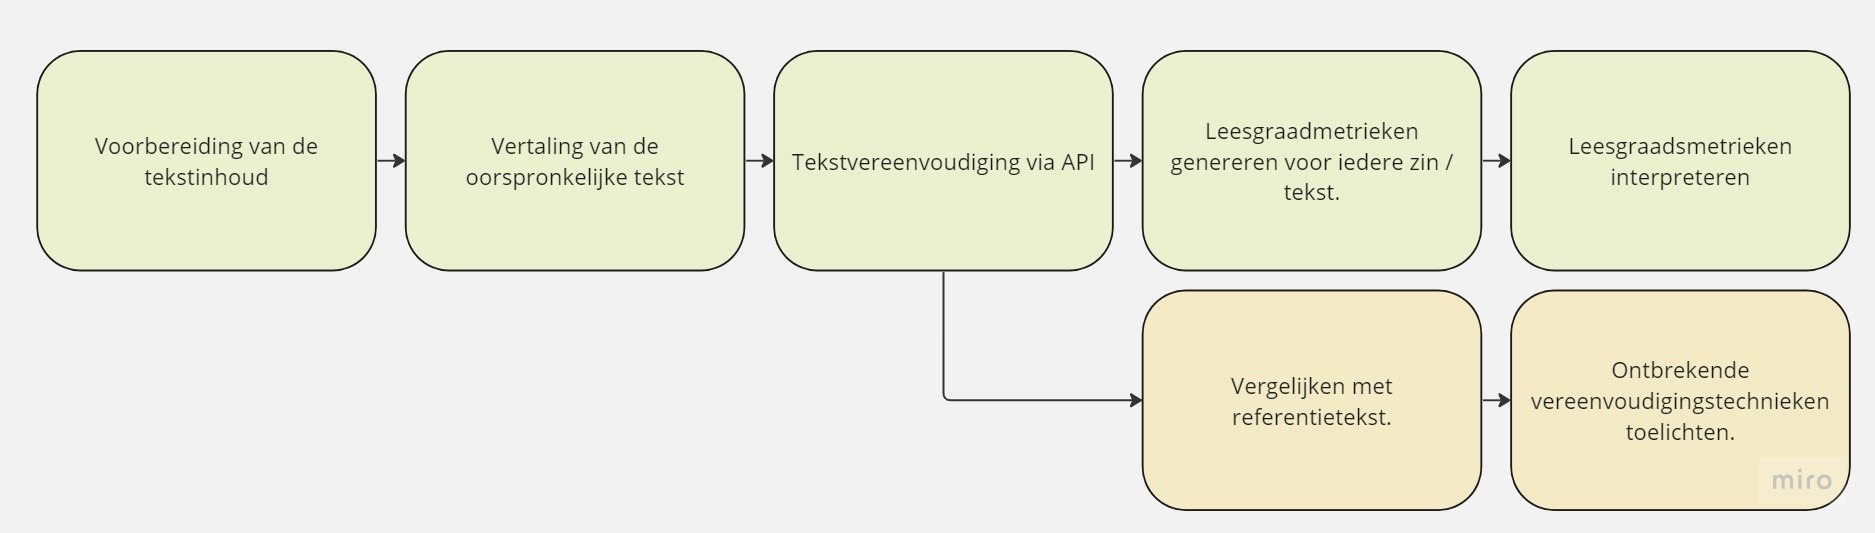
\includegraphics[width=\linewidth]{img/flowchart-vergelijkende-studie.jpg}
\caption{Het gevolgde stappenplan voor de vergelijkende studie.}
\label{img:flowchart-vergelijkende-studie-metrics}
\end{figure}

\medspace

% SCRIPT 1
Eerst volgt er een voorbereiding van de tekstinhoud. Allereerst haalt het script de inhoud van de map met wetenschappelijke artikelen op om deze vervolgens in een tekstbestand te plaatsen, zoals weergegeven in codeblok \ref{code:verg-studie-phase-1}. Vervolgens vertaalt het script de zinnen in het oorspronkelijk bestand naar het Engels. Het script, verwezen in script \ref{code:verg-studie-phase-2}, doorloopt alle tekstbestanden en vertaalt de tekstinhoud met de \textit{deep\_translator} Python-bibliotheek. Zo bekomt het script een csv-bestand met daarin twee kolommen: alle Nederlandstalige en alle vertaalde Engelstalige zinnen van één wetenschappelijk artikel. Als separator gebruikt het csv-bestand een \textit{pipe}-symbool.

\medspace

Na de vertaalfase spreekt het script de taalmodellen aan om de inhoud van de wetenschappelijke artikelen te vereenvoudigen, weergegeven in code \ref{code:verg-studie-phase-3}. Allereerst vindt een tokenisatiefase plaats. Zo gebruikt het script de tokenisatie van Spacy en de verwante embeddingsmodellen weergegeven in tabel \ref{table:wordembeddings-spacy}. Daarna vinden de API-calls plaats. API-calls in de \textit{scientific\_simplify}-functie naar HuggingFace of OpenAI regelen de taalverwerking. De request naar de HuggingFace API bestaat uit de parameters weergegeven in tabel \ref{table:huggingface-requests-parameters}. Alle taalmodellen via de API vereisen een laadfase en daarom krijgt de \textit{API-call} een extra parameter, namelijk \textit{wait\_for\_model}. Verder past dit script geen extra parameters van de taalmodellen aan. Tabel \ref{table:tested-prompts} visualiseert de gebruikte prompts voor de testen bij het GPT-3 model. Zowel T1 als T4 maken gebruik van een \textit{nul-temperature} en een \textit{top-p} waarde van 90\% om zo een probabilisch vertrouwd antwoord te krijgen, net als om een hoge woordfrequentie te krijgen zoals aangegeven in \ref{table:gpt-3-parameters}. Bij T1 zijn deze parameters ingebakken. Nadien verwerken de taalmodellen iedere zin uit de tekst. Ten slotte beantwoordt de HuggingFace of GPT API in JSON-formaat, bevattende de vereenvoudigde versie van de opgegeven zin. T1, T2 en T3 vereenvoudigen de Engelstalige zinnen, in tegenstelling tot T4 en verwante prompts die de Nederlandstalige zinnen vereenvoudigen. Zoals aangehaald kunnen prompt-gebaseerde testen verschillende resultaten krijgen, afhankelijk van de gegeven input. Daarom gebruikt het script drie verschillende prompts, gebaseerd op de tekstvereenvoudigingstechnieken beschreven in tabel \ref{table:manual-simplification}. Om een \textit{request failure} door een te lange input te voorkomen, breekt het script de volledige input op per 1000 tokens.


\begin{center}
	\begin{table}[H]
		\begin{tabular}{ | m{7cm} | m{7cm} | } 
			\hline
			\textbf{Taal} & \textbf{Embeddingsmodel} \\
			\hline
			Nederlands & NL Core News Medium\footnote{https://github.com/explosion/spacy-models/releases/tag/nl_core_news_md-3.5.0} \\ 
			\hline
			Engels & EN Core Web Medium\footnote{https://github.com/explosion/spacy-models/releases/tag/en_core_web_md-3.5.0} \\
			\hline
		\end{tabular}
		\caption{Gebruikte SpaCy word-embeddings}
		\label{table:wordembeddings-spacy}
	\end{table}
\end{center}

\begin{center}
	\begin{table}[H]
		\begin{tabular}{ | m{6cm} | m{8cm} | } 
			\hline
			\textbf{Naam parameter} & \textbf{Waarde} \\
			\hline
			Inputs & De oorspronkelijke zin. Enkel bij T1 komt 'simplify:' voor deze zin. \\
			\hline
			Max length & De lengte van de oorspronkelijke zin + 10 tokens. \\
			\hline
			Wait for model & Altijd ingesteld op \textit{True}. \\
			\hline
		\end{tabular}
		\caption{Meegegeven parameters bij HuggingFace-requests}
		\label{table:huggingface-requests-parameters}
	\end{table}
\end{center}

\begin{center}
	\begin{table}[H]
		\begin{tabular}{ | m{2cm} | m{13cm} | } 
			\hline
			\textbf{Naam} & \textbf{Prompt} \\
			\hline
			P1 & Vereenvoudig deze tekst \\
			\hline
			P2 & Vereenvoudig deze tekst voor studenten (16-18 jaar) door moeilijke woorden te vervangen, vakjargon te schrappen, woorden langer dan 18 letters te vervangen, acroniemen voluit te schrijven, een woord slechts eenmaal door een synoniem te vervangen, korte uitleg te geven wanneer dat nodig is, en percentages te vervangen. \\
			\hline
			P3 & Vereenvoudig een tekst door deze op te delen in kortere zinnen van maximaal tien woorden. Verander voornaamwoorden als 'zij', 'hun' of 'hij' in namen. Vervang complexe zinsconstructies en voorzetselzinnen door eenvoudiger alternatieven, maar laat ze ongewijzigd als er geen eenvoudiger optie beschikbaar is. \\
			\hline
		\end{tabular}
		\caption{De GPT-3-prompts die in de vergelijkende studie aan bod komen.}
		\label{table:tested-prompts}
	\end{table}
\end{center}


Vervolgens berekent het script leesgraadsmetrieken met de \textit{readability} Python-bibliotheek. Leesgraadsformules dienen, zoals aangegeven in \textcite{Nenkova2004}, als objectieve maatstaf bij deze vergelijkende studie. 

\begin{itemize}
	\item 
	\item FRE en FOG zijn relevant omdat ze de moeilijkheidsgraad van een zin of tekst objectief kunnen meten.
	\item Het aantal complexe en lange woorden kan wijzen op de gebruikte substitution generation van het taalmodel.
	\item Het aantal hulpwerkwoorden en vervoegingen van 'zijn' kan aanduiden op mogelijke passieve stem, wat eerder als hinderende taal werd gezien in de literatuurstudie door (...).
\end{itemize}




Listing \ref{code:verg-studie-phase-4} maakt een dataframe aan met de Pandas-bibliotheek. Het resultaat van dit script is een \textit{Pandas-dataframe} met alle leesbaarheidsmetrieken uit de \textit{readability}-library. Ten slotte slaat het script de \textit{Pandas-dataframe} op als CSV-bestand. In de volgende fase komt het visualiseren en interpreteren van de resultaten aan bod, waarbij een \textit{Jupyter-notebook} Matplotlib gebruikt om resultaten te visualiseren.

\begin{center}
	\begin{table}[H]
		\begin{tabular}{ | m{8cm} | m{7cm} | } 
			\hline
			\textbf{Leesgraadsmetriek} & \textbf{Vereenvoudigingstechniek }\\
			\hline
			FOG & Lexicale en syntactische vereenvoudiging \\
			\hline
			FRE & Lexicale en syntactische vereenvoudiging \\
			\hline
			Aantal woorden per zinnen & Syntactische vereenvoudiging \\
			\hline
			Aantal complexe woorden per zin volgens Dale Chall index & Lexicale vereenvoudiging \\
			\hline
			Aantal lange woorden per zin & Lexicale vereenvoudiging \\
			\hline
			Aantal gebruikte hulpwerkwoorden & Syntactische vereenvoudiging. \\
			\hline
			Aantal zinnen met een vervoeging van het werkwoord 'zijn' & Syntactische vereenvoudiging. \\
			\hline
		\end{tabular}
		\caption{De objectieve metrieken voor de vergelijking van de vereenvoudigde teksten met de oorspronkelijke tekst en de referentieteksten.}
		\label{table:verg-studie-metrieken}
	\end{table}
\end{center}

%
Tenslotte komen de resultaten van de menselijke beoordeling aan bod. Deze fase van de vergelijkende studie staat stil bij aspecten die leesmetrieken niet kunnen meten, waaronder de normen vermeld in tabel \ref{table:criteria-vergelijkende-studie-human-obv}. De referentietekst dient hier als hulpmiddel om de referentietekst, ofwel het verwachte resultaat, te vergelijken met de vereenvoudigde tekst door een taalmodel. 

\begin{table}
	\begin{tabular}{| m{6cm} | m{6cm} |}
		\hline
		\textbf{Metriek} & \textbf{Vereenvoudigingstechniek} \\ \hline
		Acroniemen behouden & Lexicale vereenvoudiging 	\\ \hline
		Inschatting van de doelgroep & Lexicale vereenvoudiging	\\ \hline
		Behoud van kern- en bijzaken & Lexicale vereenvoudiging \\ \hline
		Bronvermelding behouden &  ... \\ \hline
		Schrijven in tabelvorm of als opsomming & Structurele aanpassing \\ \hline
		Passieve zinconstructies herschrijven naar actieve zinconstructies & Syntactische vereenvoudiging \\ \hline
		Citeren en parafraseren & ... \\ \hline
	\end{tabular}
	\caption{Criteria voor menselijke observatie bij de vergelijkende studie.}
	\label{table:criteria-vergelijkende-studie-human-obv}
\end{table}

\section{Prototype voor tekstvereenvoudiging}

Met de benodigde functionaliteiten en het geschikte taalmodel voor gepersonaliseerde ATS, kan het onderzoek een volgende stap zetten richting het beantwoorden van de onderzoeksvraag. Deze sectie omschrijft de ontwikkeling van een prototype voor gepersonaliseerde tekstvereenvoudiging voor scholieren met dyslexie in de derde graad van het middelbaar onderwijs en biedt daarmee een antwoord op de volgende deelvraag: 

\begin{itemize}
	\item Hoe kan een intuïtieve en lokale webtoepassing worden ontwikkeld die zowel scholieren met dyslexie als docenten helpt bij het vereenvoudigen van wetenschappelijke artikelen met behoud van semantiek, jargon en zinsstructuren?
\end{itemize}

Deze ontwikkeling volgt de flowchart weergegeven op figuur \ref{img:general-overview-prototype}. Verder verduidelijkt figuur \ref{img:stappenplan-leerkrachten} het stappenplan voor het lerarencomponent en figuur \ref{img:stappenplan-scholars} verduidelijkt het stappenplan voor het scholierencomponent.

\begin{figure}[H]
	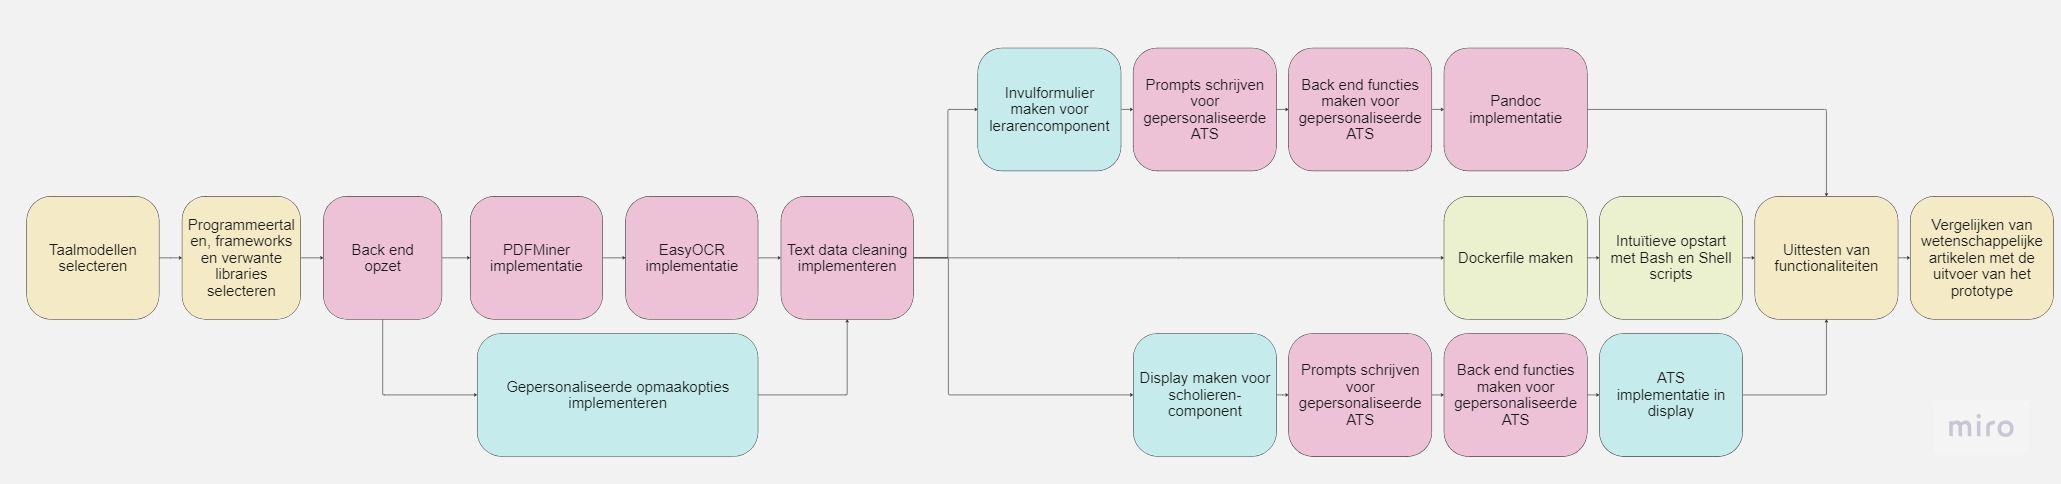
\includegraphics[width=\linewidth]{img/flowchart-general-development.jpg}
	\caption{Algemeen overzicht van de ontwikkeling van het prototype voor ATS van wetenschappelijke artikelen.}
	\label{img:general-overview-prototype}
\end{figure}

Allereerst bepaalt het onderzoek het gebruikte taalmodel voor gepersonaliseerde ATS, omdat deze keuze de beperkingen en mogelijkheden van de technologieën, zoals API-oproepen of lokale configuratie, kan beïnvloeden. Na de bepaling van het taalmodel, dat in sectie \ref{sec:vergelijkende-studie} gebeurt, wijst het onderzoek de gebruikte technologieën en frameworks voor de back-end en de front-end. Omwille van de beschikbaarheid van GPT-3 en HuggingFace-taalmodellen via API-calls, zijn Python en JavaScript geschikte keuzes voor dit prototype. Voor een snelle en gratis ontwikkeling, gebruikt het prototype open-source pakketten. Tabel \ref{table:technologies} toont een breed overzicht van alle gebruikte programmeertalen. Hierop vult tabel \ref{table:python-libraries} aan door een overzicht te geven van alle gebruikte Python-libraries.

\begin{center}
	\begin{table}[H]
	\begin{tabular}{ | m{4cm} | m{11cm} | } 
		\hline
		\textbf{Technologie} 	& \textbf{Functionaliteit} \\
		\hline
		Python 					& De back-end van het prototype die API-calls en de NLP-functionaliteiten zoals PoS-tagging en lemmatizing verwerkt. \\
		\hline
		JavaScript (JS)				& De toepassing gebruikersvriendelijker maken, personalisatie-opties voor de site doorvoeren en de functies gebouwd in Javascript dienen als alternatief op commandline instructies. \\
		\hline
		HTML en CSS 			& Het visuele uiterlijk van de website aanpassen naargelang de gekozen parameters van de eindgebruiker. \\
		\hline
		Jinja 					& Informatie uit de back-end doorgeven aan de front-end.  \\
		\hline
		Docker 					& Lokale uitrol van de webtoepassing. \\
		\hline
		Bash					& Intuïtief script om de webtoepassing op te starten voor Linux en Mac-systemen. \\
		\hline
		Powershell 				& Intuïtief script om de webtoepassing op te starten op Windows-systemen. \\
		\hline
	\end{tabular}
	\caption{Gebruikte programmeertalen in het prototype voor tekstvereenvoudiging.}
	\label{table:technologies}
	\end{table}
\end{center}

\begin{center}
	\begin{table}[H]
	\begin{tabular}{ | m{4cm} | m{11cm} | } 
		\hline
		\textbf{Python-bibliotheek} & \textbf{Functionaliteit} \\
		\hline
		Flask					& Het framework van de webtoepassing. Deze combineert front-end en back-end en past binnen de scope van een prototype. \\ 
		\hline
		PDFMiner 				& Tekstinhoud van PDF's inlezen. \\ 
		\hline
		EasyOCR					& PDF-pagina's inscannen als afbeelding in JPG-formaat om vervolgens de tekst te extraheren. \\
		\hline
		NumPy 					& De reshape-functie vereenvoudigt de manier om arrays van zinnen bij elkaar te plaatsen om zo een paragraaf te bekomen. \\
		\hline		
		Spacy 					& PoS-tagging en het lemmatiseren van woorden. \\
		\hline
		OpenAI					& GPT-3 API aanspreken. \\
		\hline
		Requests				& HuggingFace API aanspreken en informatie ophalen van een lexicale databank API. \\
		\hline
		BeautifulSoup			& HTML-content \textit{parsen} voor een correcte formatting. \\
		\hline
	\end{tabular}
	\caption{Gebruikte Python-libraries en hun respectievelijke functie in het prototype.}
	\label{table:python-libraries}
	\end{table}
\end{center}

\subsection{Ontwikkeling en personaliseerbaarheid van de webpagina's ontwikkelen}

De homepagina, weergegeven op figuur \ref{img:homepage}, biedt een kort overzicht van de twee algemene functionaliteiten, alsook instellingen waar gebruikers de webtoepassing kunnen aanpassen naargelang hun voorkeuren. Zoals aangeraden door \textcite{Harvard2023}, moeten ontwikkelaars rekening houden met de opmaakopties van de website. Deze functionaliteit gaat volgens hem vaak onopgemerkt en heeft nochtans een bewezen effect op het leesgedrag -en begrip van zowel mensen met als zonder dyslexie. De webtoepassing maakt gebruik van de standaardparameters, uitgewezen in \textcite{Rello2013a, Rello2013b}. Op een apart scherm kan de eindgebruiker de volgende elementen aanpassen naar hun toebehoren. Het prototype kan na aanpassing van de parameters eruit zien zoals weergegeven in figuur \ref{img:website-instellingen}. Met JS kunnen scholieren deze parameters \textit{on-the-spot} aanpassen. Om te voorkomen dat de eindgebruiker niet per pagina deze parameters moet instellen, verandert de back-end deze sessievariabelen aan na de aanpassing. Voor dit prototype zijn er twee soorten eindgebruikers: leerkrachten die wetenschappelijke artikelen met ATS willen vereenvoudigen op maat van scholieren en de scholieren die dit zelf willen doen.

\medspace

Voordat de ontwikkeling van het prototype deze splitsing maakt, moet de extractie van tekstinhoud uit een wetenschappelijk artikel gebeuren. Zo biedt het prototype twee manieren aan om wetenschappelijke artikelen in te laten: \textit{plaintext} of via een PDF-bestand. Het prototype hergebruikt deze functie voor het leraren- en het scholierencomponent. Echter zijn niet alle \textit{PDF extractors} foutbestendig, want zoals eerder aangewezen in tabel \ref{sec:requirementsanalyse} kunnen \textit{extractors} ook tekst niet opnemen. Als valnet biedt het prototype een OCR-optie aan. Deze functionaliteit omvat de ontwikkeling van functionaliteiten aan de front-end en aan de back-end.

\medspace

De front-end kent enkel de toevoeging van een checkbox en twee \textit{input-tags}, namelijk een \textit{file-input} en een \textit{textarea-input}. De \textit{file-input} geeft de binaries van het PDF-bestand mee van de front-end naar de back-end die het PDF-bestand tijdelijk \textit{in-memory} opslaat. Daarnaast krijgt de back-end de keuze van de gebruiker tussen normale en OCR-upload mee als boolean, waarbij 1 gelijk staat aan een OCR-afhandeling. Ten slotte gebruikt het formulier een POST-request om alle meegekregen informatie door te sturen naar de back-end. Na het ontvangen van de request van de front-end, handelt de Flask back-end het bestand verder af zoals aangewezen in listing \ref{code:inlezen-wetenschappelijk-artikel-front-end-back-end}. Eerst controleert de \textit{back-end} het type invoer. Vervolgens spreekt de Flask back-end de Reader-klasse aan die de tekst formatteert tot een bruikbaar formaat voor de webtoepassing. 

\begin{enumerate}
	\item PDFMiner itereert doorheen alle PDF-pagina's en extraheert vervolgens de tekst op iedere pagina. Deze methode resulteert in een string-object met alle geëxtraheerde tekst uit een PDF. De uitgewerkte listing staat uitgeschreven in \ref{code:inlezen-van-pdf}.
	\item De Python-bibliotheek EasyOCR voorziet een eenduidige en ontwikkelaarsvriendelijke manier om PDF-pagina's op te slaan als JPG of PNG. EasyOCR itereert doorheen alle pagina's in een PDF en slaat de pagina's op als JPG. Vervolgens leest EasyOCR de tekst op iedere pagina in en houdt dit bij tot het einde van het script. Na het inlezen van de tekst, verwijdert het script de aangemaakte afbeeldingen om zo geheugenruimte te besparen. Net zoals bij de eerste methode, resulteert deze methode in een string-object met alle tekst uit de PDF. De uitgewerkte code staat uitgeschreven in listing \ref{code:reader-ocr}
\end{enumerate}

Na het extraheren van de tekstinhoud, komt een formatteerfase aan bod waarbij het systeem de tekst omvormt naar het gewenste formaat van de gebruiker. Eerst transformeert de back-end de geëxtraheerde tekst naar arrays van zinnen met Spacy sentence embeddings. Zoals aangegeven in \ref{code:reader-formatting} staat de standaardparameter voor het aantal zinnen per paragraaf ingesteld op vijf zinnen, maar gebruikers kunnen dit aanpassen via het HTML-formulier bij de instellingen. Om de PoS-tag bij het respectievelijke woord bij te houden, gebruikt het prototype een \textit{key-value pair} datastructuur. Zo verwijst de sleutel naar een woord in een zin en de waarde verwijst naar de PoS-tag. Het prototype is ontworpen voor alleen Nederlandstalige en Engelstalige wetenschappelijke artikelen. Daarom laadt Spacy enkel twee embeddingsmodellen op, namelijk de embeddingsmodellen vermeldt in tabel \ref{table:wordembeddings-spacy}. Hardcoderen is uit den boze en daarom maakt het prototype gebruik van een \textit{dictionary} die de naam van deze embeddingsmodellen bijhoudt. Zo hoeft er enkel een taalherkenning plaats te vinden. Fouttolerantie aanbieden kan in de vorm van een standaardtaal in de dictionary, namelijk het Nederlands, of door vooraf de taal van de opgeladen tekst via een HTML-formulier aan de gebruiker te vragen.

\medspace

Zowel het leraren- als het scholierencomponent passen deze dynamische HTML-structuur binnen hun weergave toe. Zo zijn er vier verschillende klassen die aan span-tags in deze weergave worden toegekend. Door middel van een Jinja-iteratie, krijgt iedere \textit{span-tag} een specifieke klasse afhankelijk van de key of iteratie. Zo is er een overkoepelende span-tag \textit{sentence}, alsook voor ieder woord in een zin hoort er een span-tag met \textit{nouns}, \textit{adjectives} of \textit{verbs}. Andere woorden, zoals conjuncties, behoren tot de klasse \textit{other}.

\subsection{Lerarencomponent}

Na het extraheren van de tekstinhoud van een wetenschappelijk artikel, komt de ontwikkeling van de leraren- en scholierencomponeten aan bod. Zo kunnen leerkrachten beschikken over een tool waarin zij de geëxtraheerde tekstinhoud kunnen manipuleren, om vervolgens opties voor gepersonaliseerde ATS te selecteren. Figuur \ref{img:proto-lerarencomponent} toont een mogelijke weergave van deze HTML-pagina. Leerkrachten binnen dit lerarencomponent beschikken over de functionaliteiten, weergegeven in tabel \ref{table:functionaliteiten-leerkrachten}. Het HTML-formulier omvat alle benodigde tekstvereenvoudigingstechnieken op lexicaal en syntactisch niveau die tabel \ref{table:criteria-requirementsanalysis} eerder uitwees. 

\begin{center}
	\begin{table}[H]
		\begin{tabular}{ | m{7cm} | m{8cm} | } 
			\hline
			\textbf{Functionaliteit} & Gebruikte JS of Python techniek \\
			\hline
			Specifieke prompt meegeven per paragraaf & Naast een optie om voor het hele document één prompt te gebruiken, voegt het prototype ook een optie toe om. Hiervoor past de web-inhoud een key-value structuur toe. \\
			\hline
			Opties voor gepersonaliseerde ATS aanreiken. & Met behulp van een HTML-formulier kunnen leerkrachten checkboxes afvinken waaraan de gegenereerde tekst moet voldoen. Deze verschillende opties zijn terug te vinden in tabel \ref{table:criteria-requirementsanalysis}. \\
			\hline
			Werkwoorden, bijvoeglijke en zelfstandige naamwoorden markeren & Front-end aanpassing met \textit{eventlistener}. De tekstkleur van het aangeduide type woorden verandert naar het gekozen kleur. \\
			\hline
			Zinnen verwijderen & \textit{Front-end} filter aangesproken door een \textit{eventlistener}. \\
			\hline
			Woord toevoegen aan de woordenlijst & Een \textit{eventlistener} handelt de functionaliteit af door de woorden en hun zin van voorkomen tijdelijk op te slaan in een storage. Het formulier houdt dit bij en geeft het vervolgens mee bij het indienen. Deze woorden en hun respectievelijke zin van voorkomen dienen om de woordenlijst op te vullen in het gegenereerde PDF of Word-bestand. \\ 
			\hline
			Sleutel en sessieherkenning & . \\
			\hline 
		\end{tabular}
	\caption{Alle beschikbare functionaliteiten in }
	\label{table:functionaliteiten-leerkrachten}
	\end{table}
\end{center}

Leraren kunnen handmatig zinnen uit de tekst verwijderen. Hiervoor gebruikt de \textit{front-end} een \textit{eventlistener} die de aangeklikte span-tag van klasse 'sentence' uit het HTML-document verwijdert. Naast zinnen verwijderen kunnen leraren ook woorden aan een woordenlijst toevoegen. Hiervoor gebruikt de front-end een JS-script met een \textit{eventlistener} die een woord en de toebehorende zin toevoegt aan een \textit{textarea}. Deze \textit{textarea} gebruikt een \textit{pipe}-symbool als separator om nadien de text te splitsen en een array te bekomen. Om de leerkracht opties aan te reiken voor gepersonaliseerde ATS, bevat het HTML-document een formulier met keuzes aan. Dit formulier bevat alle nodige MTS-technieken uit tabel \ref{table:criteria-requirementsanalysis}. Na een POST-request krijgt de back-end deze parameters die het systeem nadien verwerkt in de prompt voor het GPT-3 taalmodel, zoals aangewezen in listing \ref{listing:gpt-class}. Leraren kunnen ook het uitvoerbestand personaliseren met lettertypes, gekozen regeleinde, woord-spatiëring en de marge van het document. Nadat de back-end de inhoud van dit formulier ontvangt, neemt de GPT-klasse de aanvraag over. Deze klasse verwerkt drie functionaliteiten, namelijk definities en synoniemen opzoeken en gepersonaliseerde ATS.

\medspace

Allereerst dient de \textit{look-up} functie om de definitie van een woord te achterhalen. Met behulp van de prompt beschreven in listing \ref{listing:gpt-class} stuurt de Python back-end een API-call naar de GPT-3 API. Om de uitvoer zo probabilisch mogelijk te maken, gebruikt de GPT-3 API-call een \textit{nultemperature}. Tabel \ref{table:gpt-3-look-up} weergeeft de gebruikte parameters bij de API-call om een woord op te zoeken. Daarna haalt het script het verkregen antwoord uit de JSON-response om deze vervolgens tijdelijk bij te houden in een dictionary.

\begin{center}
	\begin{table}[H]
		\begin{tabular}{| m{5cm}| m{8cm} |}
			\hline
			Parameter & Gebruikte waarde \\ \hline
			Prompt & Geef een eenvoudige definitie voor '{woord}' in max 1 zin. Context {context}. \\ \hline
			Temperature & 0 \\ \hline
			Max tokens & De lengte van het woord vermeerdert met tien tokens. \\ \hline
			Model & Da Vinci 3 \\ \hline
			Top-p & 90\% \\ \hline
			Stream & False \\ \hline
		\end{tabular}
	\caption{Gebruikte parameters om de definitie van een woord te genereren met GPT-3.}
	\label{table:gpt-3-look-up}
	\end{table}
\end{center}

\medspace

Vervolgens gebruikt het prototype ook de GPT-klasse om een synoniem op te zoeken. Hiervoor spreekt de API de functie \textit{give-synonym} aan verwezen in listing \ref{listing:gpt-class}. Tabel \ref{table:gpt-3-synonym} toont een overzicht van de gebruikte parameters om de synoniem van een woord te genereren.

\begin{center}
	\begin{table}[H]
		\begin{tabular}{| m{5cm}| m{8cm} |}
			\hline
			Parameter & Gebruikte waarde \\ \hline
			Prompt & Geef een eenvoudiger synoniem voor '{woord}'. Context {context}. \\ \hline
			Temperature & 0 \\ \hline
			Max tokens & De lengte van het woord vermeerdert met tien tokens. \\ \hline
			Model & Da Vinci 3 \\ \hline
			Top-p & 90\% \\ \hline
			Stream & False \\ \hline
		\end{tabular}
		\caption{Gebruikte parameters om het synoniem van een woord te genereren met GPT-3.}
		\label{table:gpt-3-synonym}
	\end{table}
\end{center}

\medspace

Daarna komt de vereenvoudiging van zinnen aan bod. Echter moet het script rekening houden met twee aspecten. Allereerst kan de leerkracht kiezen voor een opsomming van de tekst. Daarnaast moet de inputlengte overeenstemmen met de beperkingen van de GPT-3 API. Wetenschappelijke artikelen zijn bijna altijd langer dan de mogelijk inputlengte. Daarom splitst het prototype de oorspronkelijke tekst op per 1000 tokens, zodat de inputprompt over marge beschikt en daardoor alle nodige gepersonaliseerde ATS-opties mee kan geven. Bij deze splitsing houdt het script rekening met de volledigheid van een zin. De code voor de gepersonaliseerde ATS staat weergegeven in listing \ref{listing:gpt-class}. Tabel \ref{table:gpt-3-sentence-simplification} geeft een overzicht weer van de gebruikte parameters.

\begin{center}
	\begin{table}[H]
		\begin{tabular}{| m{5cm}| m{8cm} |}
			\hline
			Parameter & Gebruikte waarde \\ \hline
			Prompt & Vereenvoudig deze zinnen op basis van {MTS-technieken} :return: Een lijst van vereenvoudigde zinnen opgesplitst door een '|' sign /// {zin} \\ \hline
			Temperature & 0 \\ \hline
			Max tokens & De lengte van de oorspronkelijke tekst, vermeerdert met 30 tokens. \\ \hline
			Model & Da Vinci 3 \\ \hline
			Top-p & 90\% \\ \hline
			Stream & False \\ \hline
		\end{tabular}
		\caption{Gebruikte parameters om zinnen te vereenvoudigen met GPT-3.}
		\label{table:gpt-3-sentence-simplification}
	\end{table}
\end{center}

\medspace

Ten slotte giet het script de \textit{plain-text} van vereenvoudigde tekstinhoud en de woordenlijsten in een PDF- of DOCX-bestand. Zo maakt de Creator-klasse PDF's en docx-documenten volgens de meegegeven opmaakopties en maakt gebruik van Pandoc via Python. De code voor deze klasse is terug te vinden in listing \ref{code:writer-klasse}. Pandoc gebruikt een tweestapsbeweging, waarbij het eerst \textit{plain-text} naar een markdownformaat omzet en vervolgens het Markdown-bestand naar een PDF of Word-document converteert. Daarvoor is een YAML-header nodig die de elementen, beschreven in tabel \ref{table:personalized-pdf-word-document-with-pandoc}, moet bevatten. Het script voegt de meegekregen instellingen toe aan de YAML-header. De verschillende functionaliteiten van deze klasse staan opgesomd in tabel \ref{table:functions-creator-class}. Om de woordenlijst aan het markdown-bestand toe te voegen, bouwt het script eerst een \textit{dictionary}-structuur op met de positie van het woord als key en als values de woord, de PoS-tag en de opgehaalde gepersonaliseerde betekenis. Het prototype moet rekening houden met homoniemen en daarom kan de key hier niet het woord zijn. Bij een lege woordenlijst komen deze bewerkingen niet aan bod. Het script slaat de vereenvoudigde tekst nadien op in een \textit{dictionary}-structuur. Vervolgens print het script de vereenvoudigde tekst uit naar het markdown-bestand door alle titels van de \textit{dictionary}-structuur te doorlopen. Een titel uitprinten in markdown syntax moet voorafgaan aan twee \textit{hashtags}, gevolgd door een \textit{breakline}. Na de titel print het script de vereenvoudigde tekst per paragraaf uit. Bij een opsomming gaat een asterisk-symbool vooraf. Vervolgens converteert Pandoc het Markdown-bestand naar een PDF-bestand gebouwd met de XeLateX engine of een Word-bestand met de meegekregen binaries. Functie \textit{create-pdf} in listing \ref{code:writer-klasse} bouwt deze documenten op. Hoewel Flask maar één bestand kan teruggeven, comprimeert het script met de \textit{zipfile} bibliotheek deze twee bestanden tot één bestand. Zo krijgt de eindgebruiker alsnog zowel het docx- als het PDF-document. 

\begin{table}[H]
	\begin{tabular}{ | m{5cm}| m{5cm} | }
		\hline
		\textbf{Label in YAML-header} & \textbf{Voorbeeldwaarde} \\ \hline
		Title & Surveillance met artificiële intelligentie. \\ \hline
		Mainfont & Arial \\ \hline 
		Titlefont & Arial Black \\ \hline
		Date & 14-06-2023 \\ \hline 
		Document & Article \\ \hline
		Margin & 3cm \\ \hline
		Word-spacing & 0.3cm \\ \hline 
		Lineheight & singleheight \\ \hline
	\end{tabular}
	\caption{Benodigde labels voor een gepersonaliseerd document met Pandoc.}
	\label{table:personalized-pdf-word-document-with-pandoc}
\end{table}

\begin{table}[H]
	\begin{tabular}{ | m{5cm}| m{10cm} | }
		\hline
		Naam van de functie & Functionaliteit \\ \hline
		Create header & De nodige YAML-header voor het markdown-bestand aanmaken. \\ \hline
		Generate glossary & Een woordenlijst aanmaken. \\ \hline
		Generate summary & Deze functie vult het markdown-bestand met de vereenvoudigde tekst, gesplitst door de titels die de leerkracht heeft gekozen. \\ \hline
		Generate summary with summation & Indien de leerkracht een opsomming wenste, dan dient de titel nog steeds al separator, maar het script print de zinnen uit als opsomming conform aan de Markdown-syntax. \\ \hline
		Create PDF & De functies gebruikt alle bovenstaande functies indien nodig en maakt de PDF- en Word-bestanden. Nadien zal de functie de twee bestanden comprimeren tot één zip-bestand. \\ \hline
	\end{tabular}
	\caption{De gebruikte functies in de Creator-klasse.}
	\label{table:functions-creator-class}
\end{table}

\subsection{Scholierencomponent}

De taken van de \textit{NLP engineer} blijven vrijwel identiek, daarmee verwijst dit onderdeel terug naar tabel \ref{table:tasks-nlp-engineer}. Daarnaast vallen de taken van de \textit{system engineer} in dezelfde lijn als de taken bij het lerarencomponent en verwijst daarmee naar de taken verwezen in tabel \ref{table:tasks-system-engineer}. Figuur \ref{img:stappenplan-scholars} toont een stappenplan voor de ontwikkeling van het scholierencomponent.

\medspace

HTML, CSS en Jinja vormen de bouwstenen voor deze webpagina. De algemene weergave van dit component lijkt als dat van de uitgeteste chatbots, maar is hier afgetoetst op de benodigde opmaakopties verwezen in tabel \ref{table:dyslexia-necessaries}. Net zoals bij het lerarencomponent, moet het prototype een oorspronkelijke weergaven van het wetenschappelijk artikel kunnen tonen. 

\medspace

De front-end beschikt al over de PoS-tags en daarmee kan de gebruiker zelf kleuren selecteren om specifieke woorden te markeren. Adjectieven uit de tekst verwijderen is mogelijk zonder taalmodel. Zo hoeft enkel een JS-functie alle span-tags uit de verwante klasse uit te filteren, aangezien de PoS-tag bij ieder woord wordt bijgehouden.

\medspace

Scholieren kunnen weergegeven tekst markeren met hun cursor om deze vervolgens te vereenvoudigen op maat van hun noden. Zo kan de webpagina, waarbij een scholier een opsomming wilt van een tekst, eruit zien zoals in figuur \ref{img:proto-scholieren-step-1} en figuur \ref{img:proto-scholieren-step-3}. Eerst slaat JS de gemarkeerde tekst en meegekregen ATS-opties op en geeft deze door aan de back-end met een API-call. Vervolgens verwerkt de back-end deze aanvraag door een nieuwe aanvraag te sturen naar GPT-3, met daarin een prompt die de tekst en de gekozen ATS-technieken bevat. Als de tekst doorlopend is, dan verwerkt JS dit resultaat als een p-tag. Als de scholier eerder koos voor een opsomming, dan wordt er in de prompt ook expliciet een formaat verwacht. Op basis van dit formaat wordt er een ul-tag aangemaakt waarin de array van zinnen wordt geitereerd met een li-tag. 

\medspace

Scholieren kunnen zelf vragen stellen door de tekst te markeren en vervolgens op de verwante knop te drukken. Daarna stuurt een JS-call zowel de vraag van de gebruiker en de gemarkeerde tekst naar de Flask back-end. Die verwerkt de aanvraag met de functie in de zelfgemaakte GPT-klasse. Om het systeem robuust te maken, krijgt de prompt een extra veiligheidsmaatregel mee, namelijk 'op basis van deze tekst ///'. Om transparantie van het model te garanderen, geeft de back-end ook de prompt mee aan de front-end. Deze twee stappen worden afgebeeld in figuur \ref{img:step-1-proto-vraagstelling} en figuur \ref{img:step-2-proto-vraagstelling}.

\subsection{Lokale opzet}

Ten slotte gebruikt het prototype Docker voor de lokale opzet. Omdat het prototype alleen API's van taalmodellen aanspreekt, werkt het prototype met één Docker-container. Listing \ref{code:dockerfile} toont de gebruikte code van de Dockerfile. Voor het opstarten van de webapplicatie moet de Docker-container eerst de benodigde word-embeddings van Spacy installeren. Een scriptbestand in Powershell, zoals weergegeven in \ref{code:shell-boot}, of Bash zoals weergegeven in \ref{code:bash-boot}, maakt de opstart van deze webapplicatie intuïtiever dan via commandline. Het Pipreq-commando maakt een lijst van Python-bibliotheken die Docker vooraf moet installeren.